\subsection{PPO-based parameter control}
\label{sec:ppo}

Although GVNS+ provides a stronger optimization backbone than the original GVNS, its overall behaviour still depends on a set of manually calibrated hyperparameters controlling diversification, intensification, feasibility management, and stagnation recovery. In the original framework, these parameters are fixed before the search through offline calibration \cite{masmoudi2025generalized}. However, the most appropriate parameter configuration may vary significantly throughout the optimization process. Early search stages often benefit from stronger diversification, whereas later stages generally require more intensive exploitation around promising regions of the search space.

To address this limitation, we introduce a reinforcement learning controller based on Proximal Policy Optimization (PPO) \cite{schulman2017proximal}. Unlike the operator-selection agents presented previously, which act locally inside the B-VND procedure, the PPO controller operates at the global level of the metaheuristic by dynamically adapting the main search-control parameters during optimization.

%% ========= MDP formulation =========
\subsubsection{MDP Formulation}
The adaptive hyperparameter control problem is modeled as a Markov Decision Process (MDP). At each decision point, the controller observes the current optimization context, selects a search-control action, and receives a reward reflecting the impact of the resulting parameter configuration on search performance.

%% state represententaion
\paragraph{State representation}
The controller relies on the unified search-state representation introduced in Section~\ref{sec:learninginfra}. The state combines instance-level descriptors, dynamic search indicators, solution-structure characteristics, and neighborhood-context information.

In addition, the current values of the controlled hyperparameters are included in the observation vector. This allows the policy to reason jointly about the optimization state and the current search configuration. The resulting state can be expressed as

\[
s_t=
[x_t^{inst},
x_t^{search},
x_t^{sol},
x_t^{neigh},
x_t^{ctrl}]
\]

where the last component corresponds to the current parameter values.

%% action space
\paragraph{Action space}
Rather than directly predicting numerical parameter values, the controller selects among a set of high-level search behaviours. Each action modifies several parameters simultaneously and corresponds to a meaningful optimization strategy.

The controller regulates four key components of GVNS+:

\begin{itemize}
\item shaking intensity,
\item acceptance threshold,
\item penalty adaptation scale,
\item stagnation threshold.
\end{itemize}

To avoid unstable parameter oscillations, updates are smoothed using an inertia mechanism:

\[
\theta_{new}
=
0.7\theta_{current}
+
0.3\theta_{target}.
\]

The resulting values are subsequently clipped to predefined safety ranges.

\begin{table}[ht]
\centering
\caption{Safety ranges for the PPO-controlled hyperparameters.}
\label{tab:ppo_ranges}
\begin{tabular}{lcc}
\hline
Parameter & Lower bound & Upper bound \\
\hline
Shaking scale ($D_p$) & 0.3 & 1.0 \\
Acceptance threshold ($\delta$) & 0.0 & 0.4 \\
Penalty scale ($\alpha$) & 0.1 & 2.0 \\
Stagnation limit ($Cont_{max}$) & 5 & 50 \\
\hline
\end{tabular}
\end{table}

The complete action space is summarized in Table~\ref{tab:ppo_actions}. Each action corresponds to a distinct search behaviour ranging from aggressive diversification to feasibility reinforcement and stagnation recovery.

\begin{table*}[ht]
\centering
\caption{Action space of the PPO controller.}
\label{tab:ppo_actions}
\begin{tabular}{cll}
\hline
Action & Behaviour & Main effect \\
\hline
0 & Neutral stabilization &
Restore moderate baseline parameters \\

1 & Strong diversification &
Increase shaking intensity and relax acceptance \\

2 & Mild diversification &
Slightly increase shaking intensity \\

3 & Mild intensification &
Reduce shaking intensity and tighten acceptance \\

4 & Strong intensification &
Strong reduction of shaking and stricter acceptance \\

5 & Strong feasibility reinforcement &
Increase penalty pressure on constraint violations \\

6 & Mild feasibility reinforcement &
Slight increase of penalty pressure \\

7 & Stagnation reset &
Reset parameters to escape local optima \\

\hline
\end{tabular}
\end{table*}

%% reward function
\paragraph{Reward function}

The reward is designed to measure the quality of the selected parameter configuration while maintaining numerical stability during policy optimization.

Let $F_{before}$ and $F_{after}$ denote the penalized objective values before and after the corresponding local-search step. The relative improvement is computed as

\[
r_{imp}
=
\frac{F_{before}-F_{after}}
{\max(1,F_{before})}.
\]

To reduce sensitivity to extreme values, the improvement is transformed using

\[
r_{base}
=
\tanh(3r_{imp}).
\]

Additional shaping terms reward improving moves and newly discovered best solutions while slightly penalizing non-improving decisions. The final reward is clipped to the interval $[-1,1]$.

This formulation provides stable learning signals while preserving sensitivity to meaningful improvements in solution quality.

%% ========= Architecture =========
\subsubsection{PPO Controller Architecture}

The controller is implemented as a compact actor--critic neural network. Since the state representation is already engineered and normalized, a lightweight architecture is sufficient and avoids unnecessary model complexity.

The network consists of two fully connected hidden layers of 128 neurons with ReLU activations. These layers produce a shared latent representation

\[
h=f_{\theta}(s).
\]

Two output heads are then derived from this representation.

The actor head produces a probability distribution over the eight control actions:

\[
\pi(a|s)=
\mathrm{softmax}(W_{\pi}h).
\]

The critic head estimates the state value

\[
V(s)=W_v h.
\]

The actor is responsible for selecting parameter-control actions, whereas the critic estimates the expected future return and serves as a baseline for variance reduction during training.

\begin{figure}[ht]
\centering
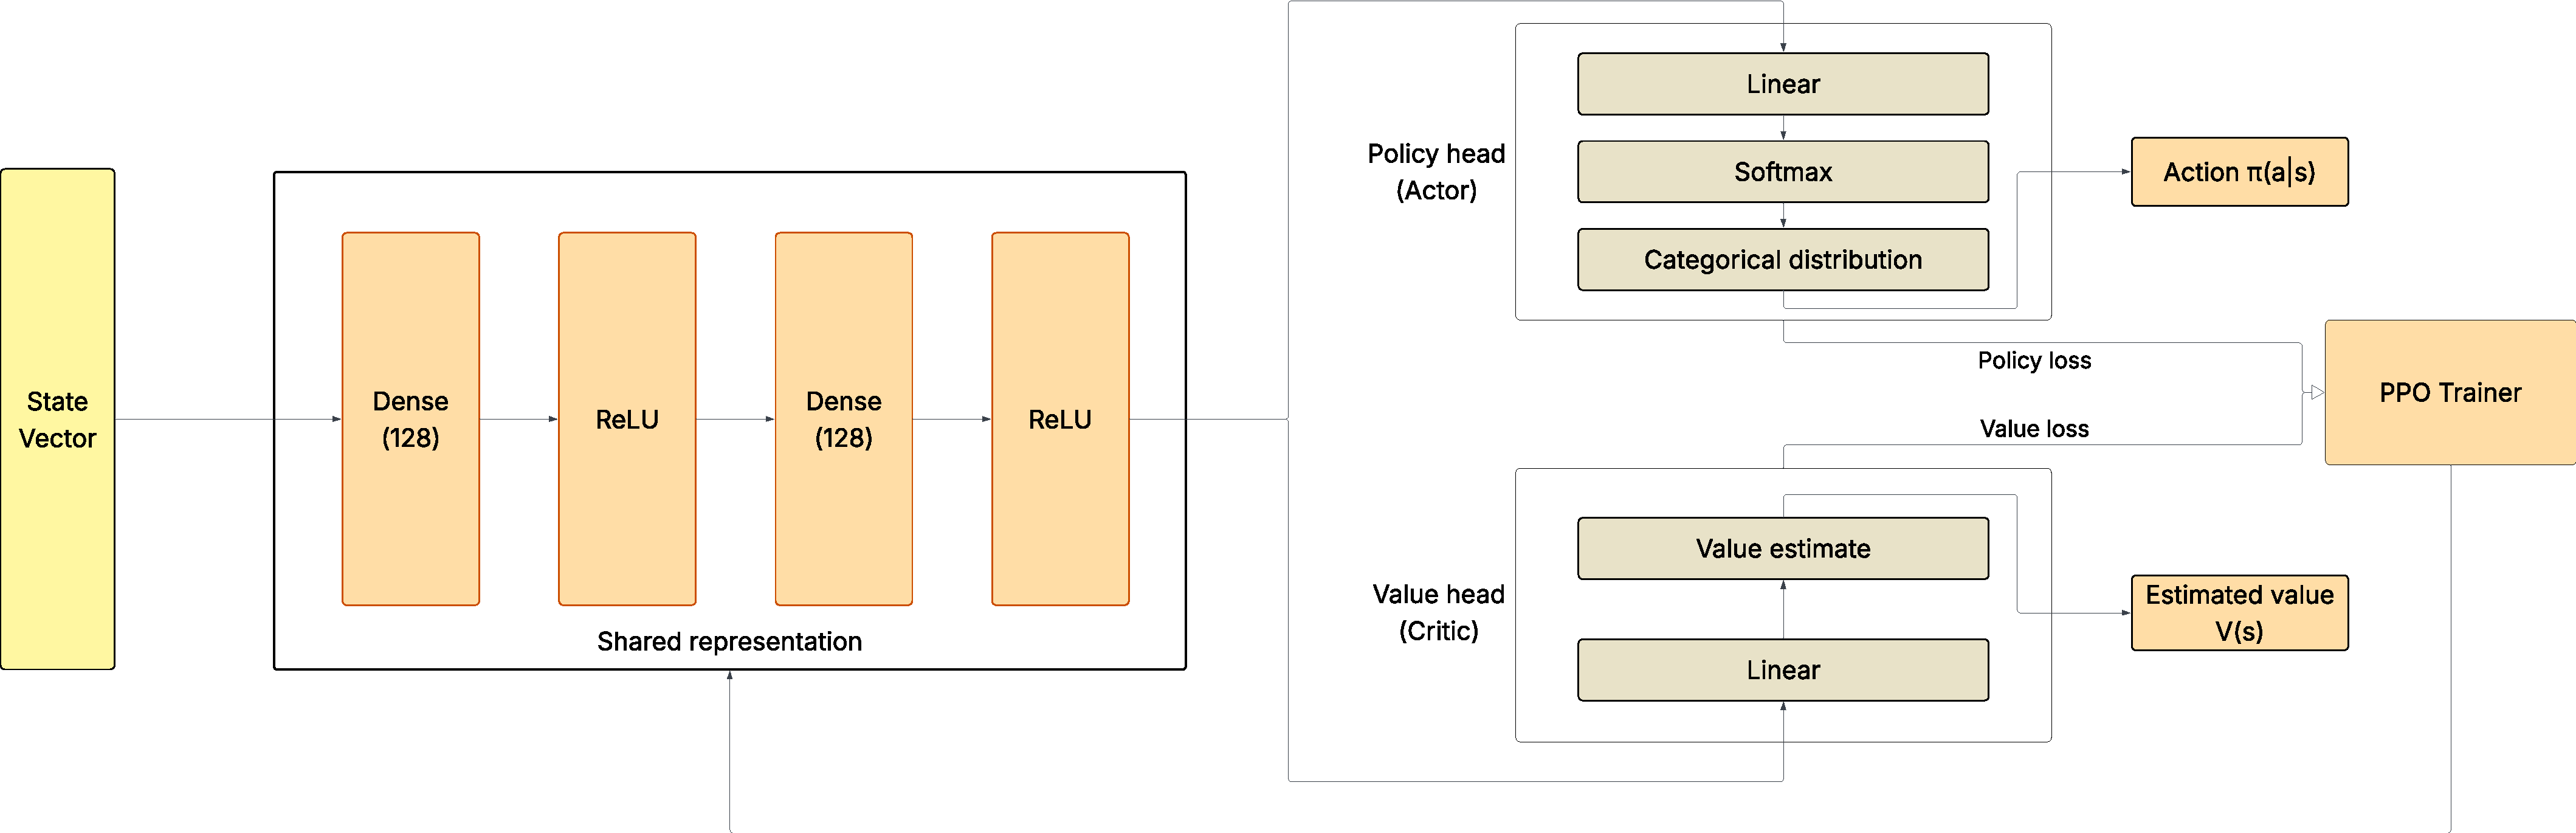
\includegraphics[width=\linewidth]
{../figures/ppo_architecture.pdf}

\caption{PPO architecture}
\label{fig:ppo_architecture}
\end{figure}

%% ========= Training =========
\subsubsection{Offline Policy Training}

Training data are obtained from the learning infrastructure presented previously. During repeated executions of GVNS+, optimization trajectories are recorded as sequences of transitions

\[
(s_t,a_t,r_t,s_{t+1}).
\]

The PPO controller is subsequently trained offline using these trajectories.

For each trajectory, discounted returns are computed according to

\[
G_t=r_t+\gamma G_{t+1},
\]

with $\gamma=0.99$. Advantages are then estimated as

\[
A_t=G_t-V(s_t).
\]

The policy is optimized using the clipped PPO objective proposed by Schulman et al.~\cite{schulman2017proximal}, while the critic is trained through mean squared error regression on the estimated returns. An entropy regularization term is additionally included to encourage exploration during learning.

Figure~\ref{fig:ppo_training_pipeline} summarizes the complete offline training workflow.

\begin{figure}[ht]
\centering
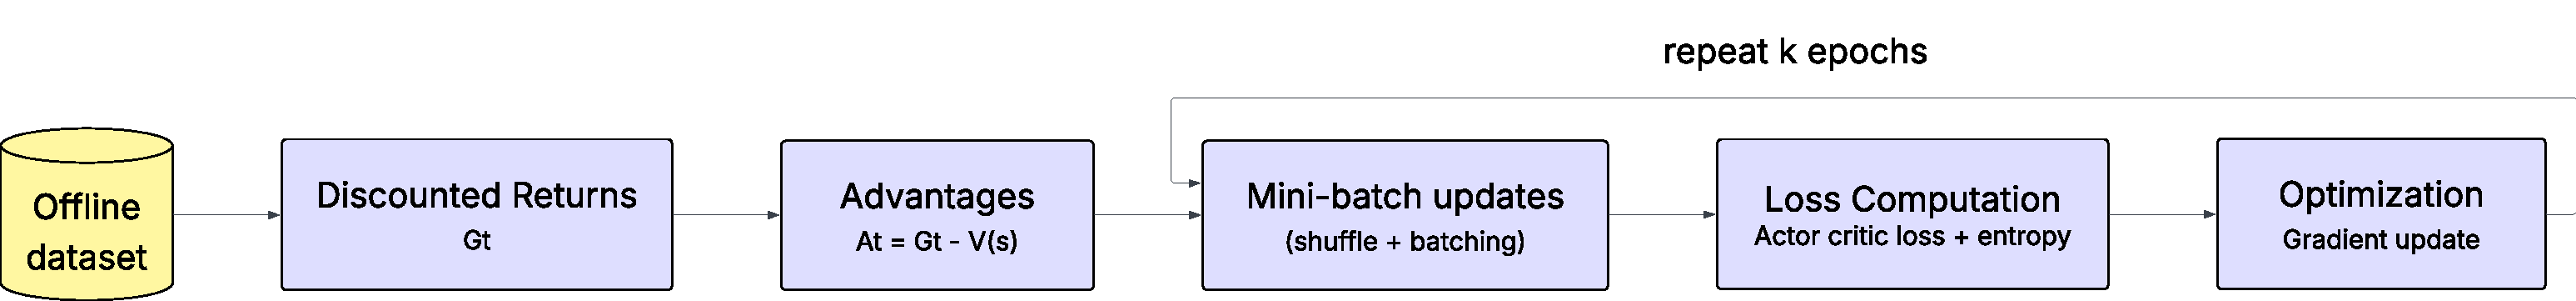
\includegraphics[width=\linewidth]
{../figures/ppo_training_pipeline.pdf}

\caption{PPO training pipeline}
\label{fig:ppo_training_pipeline}
\end{figure}

%% ========= Integration into GVNS+ =========
\subsubsection{Integration into GVNS+}

During optimization, the controller operates as a global adaptation layer placed above the standard GVNS+ search process.

At each neighborhood evaluation, the current search-state vector is extracted and provided to the PPO policy. The selected action updates the search-control parameters, after which the corresponding local-search phase is executed using the new configuration. The resulting optimization outcome is then used to compute the reward and update the search state.

Unlike static parameter calibration, this mechanism continuously adapts the search behaviour according to the current optimization context. The controller therefore regulates the balance between diversification, intensification, feasibility restoration, and stagnation recovery throughout the entire search trajectory.

Algorithm~\ref{alg:ppo_gvns} presents the overall integration of the controller within GVNS+, while Algorithm~\ref{alg:ppo_local_search} details the PPO-guided local search procedure.

\begin{algorithm}[H]
\caption{GVNS with PPO-Driven Local Search}
\label{alg:ppo_gvns}
\begin{algorithmic}[1]

\Require Instance, time limit, PPO controller
\Ensure Best solution found

\State $S \gets \Call{GenerateInitialSolution}{}$
\State $stagnation \gets 0$

\While{\Call{TerminationCondition}{time limit, stagnation} = false}

    \State Update controller parameters

    \State $S \gets \Call{Shake}{S,\ shakingScale}$
    
    \State $S' \gets
        \Call{LocalSearchWithPPO}
        {S,\ PPOController}$

    \If{$\Call{Acceptance}{S,S',\delta}$}

        \State $S \gets S'$
        \State $stagnation \gets 0$

    \Else

        \State $stagnation \gets stagnation + 1$

    \EndIf

    \State \Call{UpdatePenalties}{$S,\alpha$}

\EndWhile

\State \Return $S$

\end{algorithmic}
\end{algorithm}



\begin{algorithm}[H]
\caption{PPO-Guided Local Search}
\label{alg:ppo_local_search}
\begin{algorithmic}[1]

\Require Solution $S$, PPO controller
\Ensure Improved solution $S$

\For{each neighborhood $N_i$}

    \State $state \gets
    \Call{ExtractFeatures}{S,i}$

    \State $action \gets
    \Call{SelectAction}{state}$

    \State \Call{ApplyAction}{action}

    \State $F_{\text{before}}
        \gets
        \Call{Objective}{S}$

    \State $candidate \gets
        \Call{ApplyNeighborhood}
        {S,N_i}$

    \State $F_{\text{after}}
        \gets
        \Call{Objective}{candidate}$

    \State $improved
        \gets
        (F_{\text{after}} < F_{\text{before}})$

    \State $reward \gets
        \Call{ComputeReward}
        {F_{\text{before}},
         F_{\text{after}},
         improved}$

    \State $nextState \gets
        \Call{ExtractFeatures}
        {candidate,i}$

    \State \Call{StoreTransition}
        {state,
         action,
         reward,
         nextState}

    \If{$improved$}

        \State $S \gets candidate$

    \EndIf

\EndFor

\State \Return $S$

\end{algorithmic}
\end{algorithm}

